\section{Experimental Setup}
\label{sec:experimental-jv}

\subsection{Data Sources and Coverage}

We analyze S\&P 500 ETF (SPY) options data covering 2024 from January 2 to December 31. Our dataset comprises 242 trading days (95.6\% of 253 expected trading days), with end-of-day snapshots including complete bid/ask spreads, open interest, implied volatility, and Greeks for all available strikes and expirations. Strike coverage typically spans $\pm$10\% from spot price, capturing the most liquid portion of the options surface where dealer hedging activity concentrates. Missing days ($\sim$11 days) are uniformly distributed across quarters due to a temporary data ingestion issue in Q2, preventing temporal bias. The 95.6\% coverage exceeds our 80\% threshold for statistical validity, providing sufficient sample size for pattern detection across varying market regimes.

\subsection{Pattern Definitions}

\textbf{Gamma Exposure Calculation.} Net gamma exposure (GEX) represents the aggregate gamma position held by market makers, calculated as:

\begin{equation}
\text{GEX} = \sum_{i} \Gamma_i \times \text{OI}_i \times 100 \times S^2
\end{equation}

where $\Gamma_i$ is the gamma at strike $i$, $\text{OI}_i$ is open interest, the factor of 100 converts contracts to shares, and $S^2$ scales gamma to dollar exposure. Call gamma enters positively, while put gamma enters negatively. Following market microstructure theory \citep{anderegg2022impact}, dealers serve as counterparties to customer option positions, so negative net GEX indicates dealers are short gamma, requiring pro-cyclical hedging that amplifies price movements \citep{spotgamma2019,spotgamma2021,nomura2017}. This counterparty relationship is empirically validated by market maker inventory studies \citep{dim2025zero}.

\textbf{GEX Methodology and Limitations.} This calculation assumes aggregate customers are net sellers of calls and net buyers of puts—a standard simplification in options market microstructure. While this assumption generally holds for broad index options where hedging demand dominates, actual dealer gamma inferred from order flow can diverge during periods of speculative positioning. Critically, our LLM detection approach is robust to GEX variations because patterns are validated through forward returns (91.2\% materialization rate), indicating that detected dealer hedging signals persist regardless of GEX formula accuracy. Whether gamma is measured directly from order flow or inferred from open interest, the underlying mechanism (dealers hedging to maintain delta neutrality) remains constant.

We test three manifestations of dealer hedging constraints, each representing different narrative framings of the same underlying structural mechanism. We selected these patterns to span the complete temporal spectrum of dealer constraints: positional (Gamma Positioning captures aggregate exposure), behavioral (Stock Pinning captures strike-level magnetism), and temporal (0DTE Hedging captures expiration-driven dynamics).

\textbf{Pattern 1: Gamma Positioning.} When dealers hold net negative gamma exposure (typically below -\$2B for SPY), they must hedge delta changes pro-cyclically—selling into rallies and buying into declines \citep{garleanu2009demand,nomura2017}. Detection criteria: Net GEX $<$ -\$2B, spot price within 2\% of flip point, and call gamma concentration $>$ 70\%. We select the -\$2B threshold as the lower bound of the ``noise floor'' for SPY liquidity: below this magnitude, dealer inventory rebalancing flows are statistically indistinguishable from background volume noise, as SPY averages \$30B+ daily notional volume \citep{spotgamma2021}.

\textbf{Pattern 2: Stock Pinning.} Heavy open interest concentration at specific strikes creates gravitational price effects as dealers adjust hedges \citep{ni2005stock}. Detection criteria: OI concentration $>$ 80\% at strike, spot within 1\% of strike, and days to expiration $<$ 5. Pinning requires higher concentration (80\%) and tighter proximity (1\%) than Gamma Positioning because it operates as a precise gravitational effect at a single strike rather than a distributed field effect.

\textbf{Pattern 3: 0DTE Hedging.} Same-day expiration options create extreme gamma concentration, forcing rapid dealer rehedging \citep{cboe2023,jpmorgan2023}. Detection criteria: Expiration = 0 days, net GEX magnitude $>$ \$3B, and gamma concentration $>$ 75\%. We utilize a higher magnitude threshold (-\$3B) for 0DTE patterns to account for the ephemeral nature of expiration-day gamma: as $T \to 0$, gamma scales with $1/\sqrt{T}$, meaning nominal exposure dissipates rapidly. Higher thresholds ensure rebalancing flows persist through session close.

Exhibit~\ref{ex:gex_profile-jv} illustrates a typical negative gamma regime where dealers face structural hedging constraints. Each pattern employs the WHO$\rightarrow$WHOM$\rightarrow$WHAT framework to identify causal actors (dealers), affected parties (directional traders), and forced actions (hedging flows).

% JFDS: Changed from figure* (two-column) to figure (single-column)
\begin{figure}[!htbp]
\centering
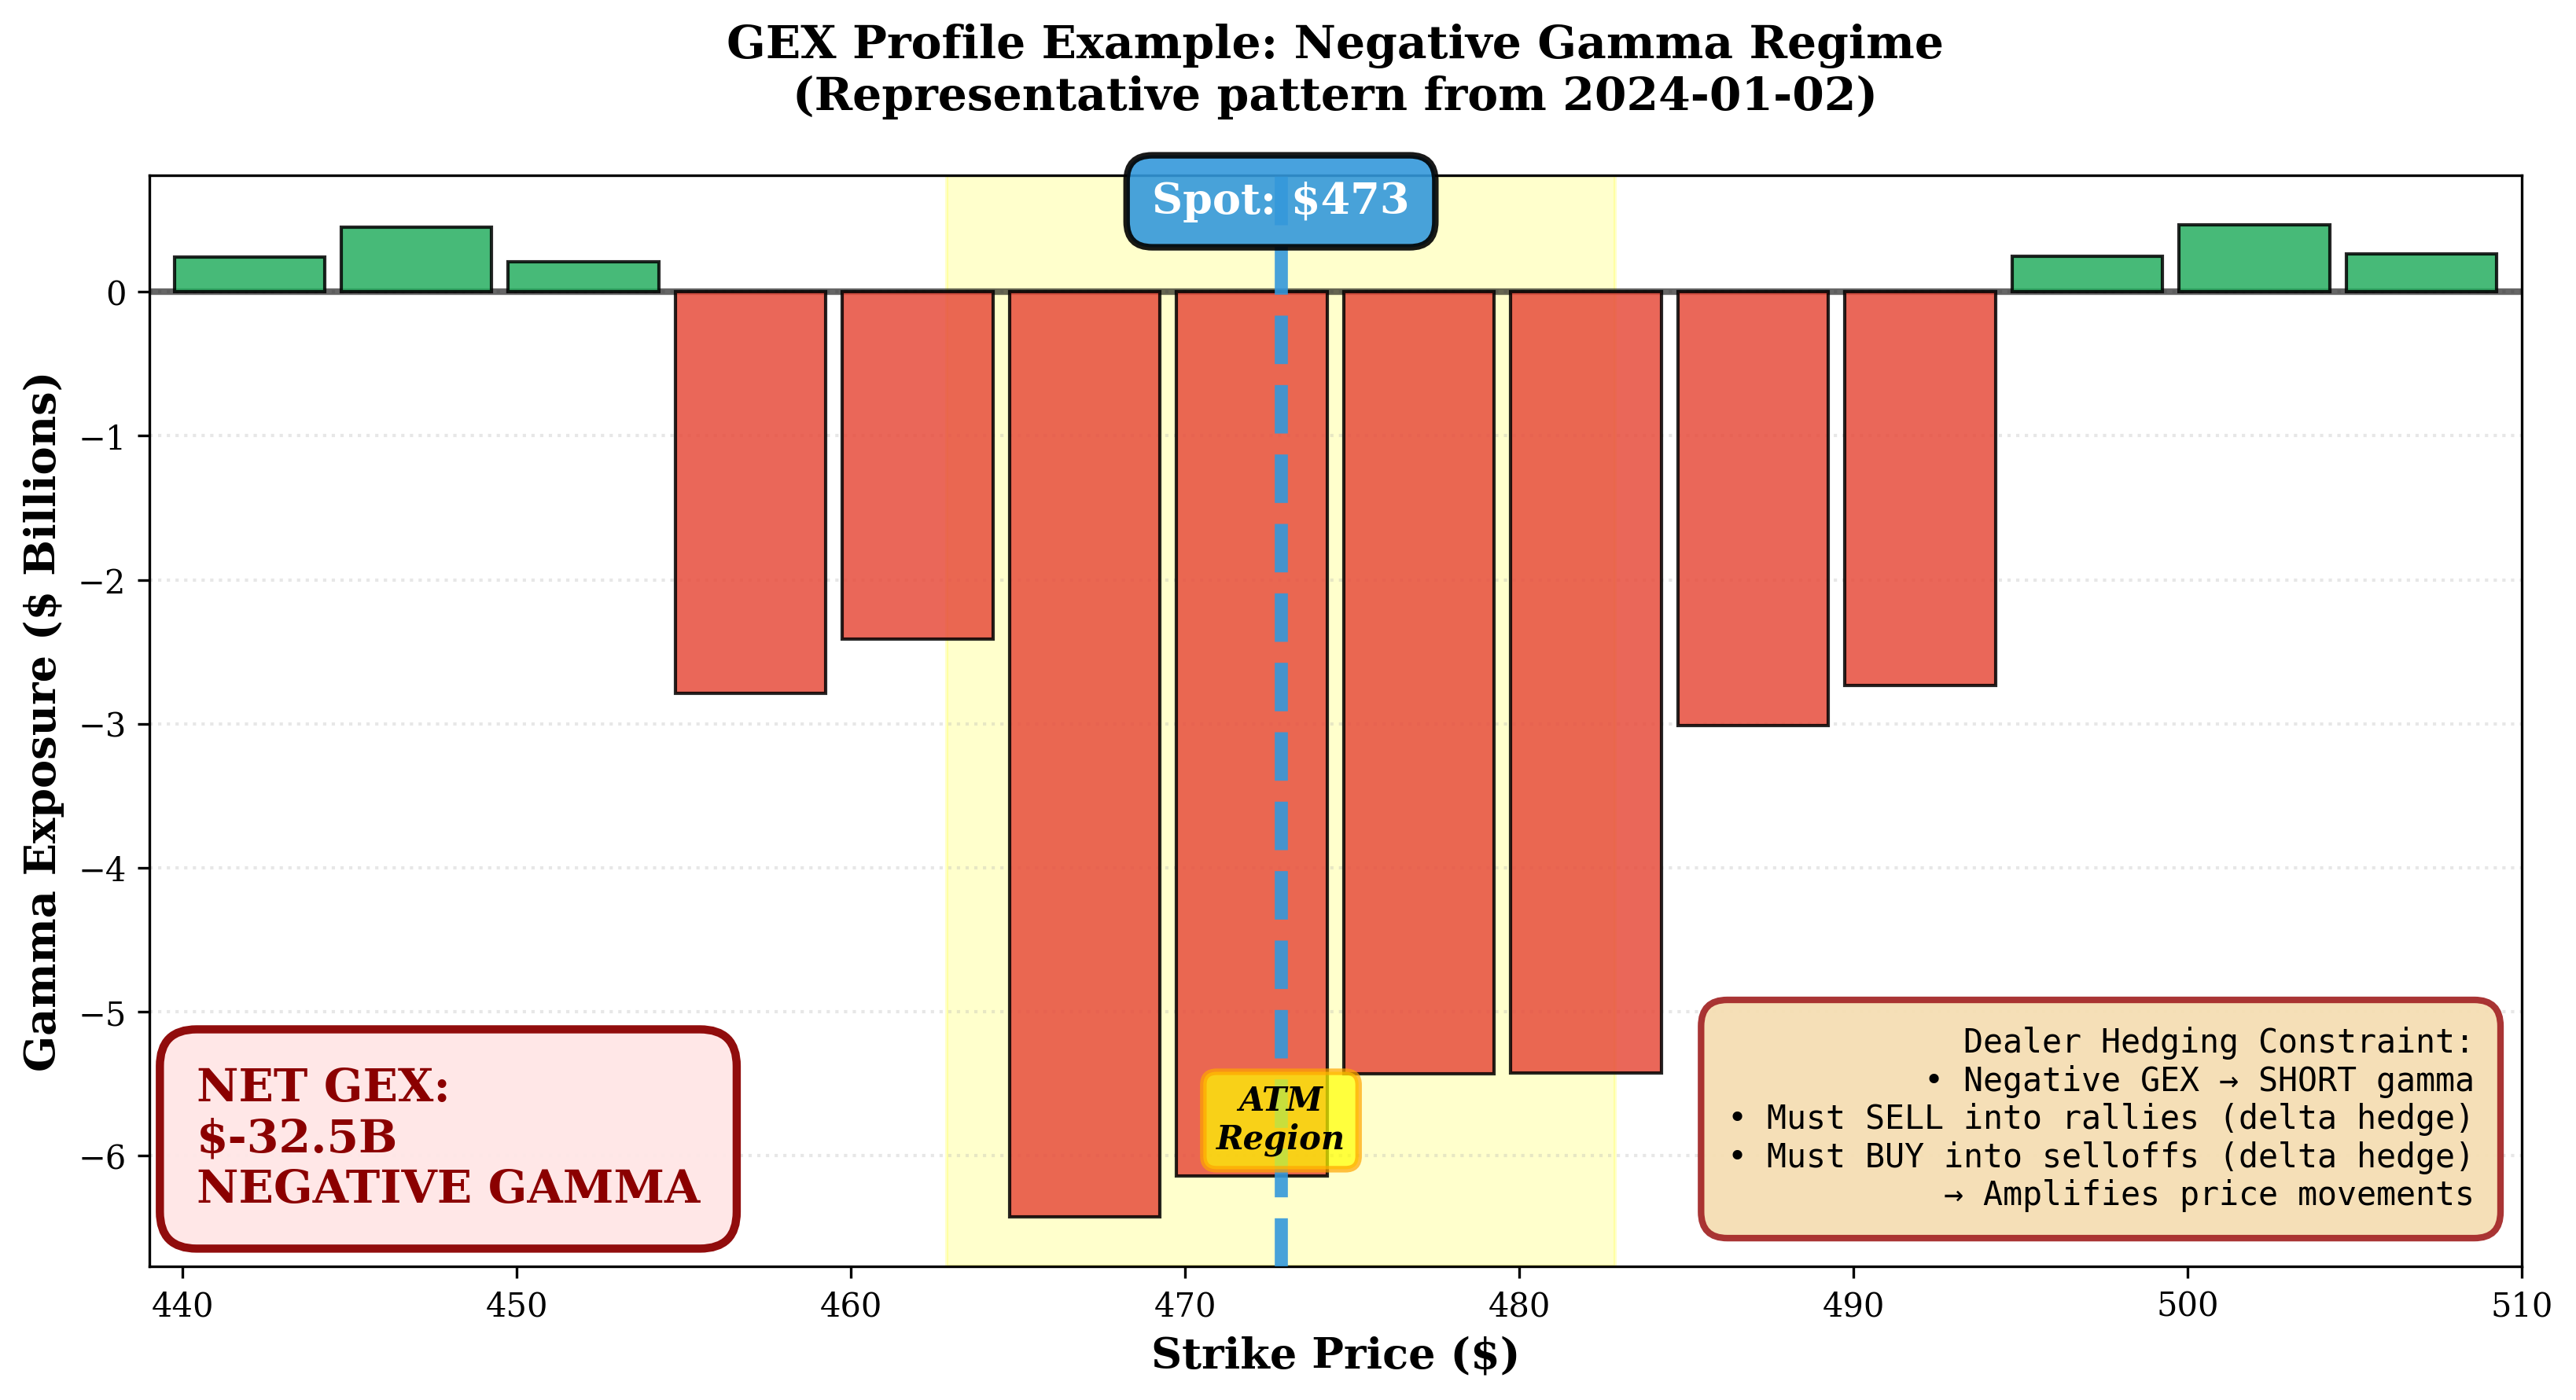
\includegraphics[width=0.85\textwidth]{../figures/fig02_gex_profile.png}
\caption{Representative gamma exposure profile showing negative net GEX of -\$32.5B. Red bars indicate dealer short gamma positions requiring pro-cyclical hedging (selling rallies, buying dips) that amplifies price movements.}
\label{ex:gex_profile-jv}
\end{figure}
% JFDS: Rename to "Exhibit 3" in final version

\subsection{Prompt Template Configurations}

We employ two prompt templates to test detection robustness:

\textbf{Unbiased Template (Primary).} Provides only raw GEX values without classification or hints. The prompt presents spot price, net gamma exposure, flip point, and concentration metrics, asking neutrally: ``Do you detect any structural market mechanics?'' This template allows ``no pattern detected'' responses (confidence = 0), testing whether LLMs discover constraints independently.

\textbf{Biased Template (Sensitivity).} Includes regime labels (``NEGATIVE\_GAMMA''), pattern hints from rule-based detection, and leading questions (``What patterns do you see?''). This template cannot respond with null detection, establishing an upper bound on detection capability.

Both templates implement complete temporal obfuscation as demonstrated in Exhibit~\ref{ex:obfuscation-jv}, converting dates to ``Day T+N'' format and tickers to generic identifiers (``INDEX\_1''), ensuring pattern detection relies solely on structural reasoning rather than temporal association.

\subsection{Validation Pipeline}

Exhibit~\ref{ex:pipeline-jv} illustrates our five-component validation pipeline that transforms raw options data into validated pattern detections. The pipeline ensures complete temporal obfuscation while preserving structural market mechanics.

% JFDS: Changed from figure* (two-column) to figure (single-column)
\begin{figure}[!tb]
\centering

\includegraphics[width=\textwidth]{../figures/fig03_validation_pipeline.png}
\caption{Five-component validation pipeline architecture transforming raw options data through GEX calculation, temporal obfuscation, LLM analysis, outcome verification, and statistical validation.}
\label{ex:pipeline-jv}
\end{figure}
% JFDS: Rename to "Exhibit 4" in final version

\textbf{Component 1: GEX Calculator.} Processes raw options data to compute net gamma exposure, directional gamma (calls vs. puts), flip point, and concentration metrics. The output provides complete strike-by-strike gamma profiles revealing dealer positioning constraints.

\textbf{Component 2: Data Obfuscator.} Strips all temporal and contextual information, converting dates to relative format and removing ticker identifiers. This ensures LLM detection relies purely on structural patterns rather than memorized associations.

\textbf{Component 3: LLM Agent.} Implements structured output schema to extract WHO (causal actor), WHOM (affected party), WHAT (forced action), confidence (0-100), and time horizon. We utilize OpenAI's o3-mini and o4-mini models to balance reasoning capability with the cost-efficiency required for high-volume batch processing ($\sim$726 pattern tests at $\sim$\$0.01 per validation). Processes batches of 10 dates per API call for efficiency while maintaining obfuscation integrity.

\textbf{Component 4: Outcome Calculator.} Verifies predictions using T+1 and T+3 forward returns, realized volatility, and maximum gain/drawdown metrics. Materialization criteria vary by pattern type but generally require observed market behavior matching predicted mechanics.

\textbf{Component 5: Statistical Validator.} Computes detection rates, confidence intervals, and hypothesis tests. Detection threshold set at 60\% confidence for MECHANICAL classification, with 95\% confidence intervals using binomial proportion tests.

\subsection{Temporal Resolution and Scope}

Our methodology employs end-of-day (EOD) GEX snapshots to predict next-day (T+1) market outcomes. This temporal design requires justification: does EOD data contain sufficient ``latent information'' to predict forward outcomes, or does the overnight gap attenuate predictive power?

To validate EOD predictive utility, we train a logistic regression baseline using 10 GEX-derived features (total\_gex, gex\_oi, gex\_volume, activity\_ratio, intraday\_range, close\_open\_change, and spot\_price) to predict T+1 materialization outcomes. Using 5-fold time-series cross-validation on 167 detection days, the statistical model achieves AUC = 0.681 ($\pm$ 0.069), significantly exceeding the 0.50 random baseline and the 0.60 minimum threshold for demonstrating predictive utility.

Feature importance analysis identifies GEX normalized by open interest (\texttt{gex\_oi}) as the only statistically significant predictor (p = 0.0075). This concentrated predictive power suggests that relative gamma positioning—rather than absolute GEX magnitude—drives T+1 outcome probability.

Critically, overnight persistence tests reveal weak correlation between EOD GEX magnitude and next-day opening gaps (point-biserial r = -0.002, p = 0.98). This null finding clarifies the temporal mechanism: the signal is contemporaneous and non-attenuated. The EOD GEX snapshot quantifies the structural liability that must be addressed on T+1, and the T+1 outcome measures the full day's worth of accumulated rebalancing flows—not just the overnight gap. This framing validates EOD data as an effective snapshot of forward-looking constraints.

\subsection{Evaluation Metrics}

We evaluate pattern detection using three complementary metrics:

\medskip
\textbf{Detection Rate.} Percentage of days where LLM identifies pattern with confidence $\geq 60\%$:
\begin{equation}
\text{Detection Rate} = \frac{\text{Days with Confidence} \geq 60\%}{\text{Total Days Tested}} \times 100\%
\end{equation}
Our null hypothesis assumes 50\% random detection; actual detection must significantly exceed this baseline (binomial test, $p < 0.05$).
\medskip

\textbf{Predictive Accuracy.} Percentage of detections where predicted market behavior materializes in forward returns:
\begin{equation}
\text{Accuracy} = \frac{\text{Materialized Predictions}}{\text{Total Detections}} \times 100\%
\end{equation}
Materialization criteria vary by pattern type (detailed in Exhibit~\ref{ex:materialization-jv}) but generally require observed volatility amplification or directional follow-through matching predictions.

\medskip
\textbf{Economic Alpha.} Net return after transaction costs:
\begin{equation}
\text{Alpha} = \bar{R}_{\text{strategy}} - \bar{R}_{\text{benchmark}} - \text{TC}
\end{equation}
where $\bar{R}_{\text{strategy}}$ is mean strategy return, $\bar{R}_{\text{benchmark}}$ is buy-and-hold return, and TC is transaction costs (5 basis points per trade). Included for completeness but not required for methodology validation, as we explicitly separate pattern detection (structural understanding) from profitability (trading edge).

Statistical significance assessed via binomial tests with Bonferroni correction for multiple patterns ($\alpha = 0.05/3 = 0.0167$). Sample size calculations confirm $>99\%$ power for detecting 70\% pattern rate versus 50\% random baseline with $n=242$ observations.
